\section{Dimensioning Video Buffer for Specific User Profiles and Behavior}\label{sec:application:qoe_user_behaviour}

\newcommand{\stallingRatio}{\ensuremath{R}\xspace}
\newcommand{\stallingDuration}{\ensuremath{L}\xspace}
\newcommand{\numberStallingEvents}{\ensuremath{N^*}\xspace}
\newcommand{\stallingFrequency}{\ensuremath{F}\xspace}
\newcommand{\meanStallingEventDuration}{\ensuremath{L}\xspace}

\newcommand{\networkBandwidth}{\ensuremath{\lambda}\xspace}
\newcommand{\playbackRate}{\ensuremath{\mu}\xspace}

\newcommand{\meanBusy}{\ensuremath{B}\xspace}
\newcommand{\meanIdle}{\ensuremath{L}\xspace}
\newcommand{\numberFrames}{\ensuremath{Z}\xspace}
\newcommand{\videoDownloadTime}{\ensuremath{t_Z}\xspace}

\newcommand{\watchLater}{\emph{Watch Later}\xspace}
\newcommand{\watchNow}{\emph{Watch Now}\xspace}
\newcommand{\videoBrowsing}{\emph{Video Browsing}\xspace}

While the previous section implicitely assumed that sufficient bandwidth for video playback is available in order to provide high \gls{QoE}, this assumption on \gls{QoS} does not always hold in the real world, for example due to a high user count in the \gls{LTE} cell, or due to difficult terrain.
Traditional \gls{QoE} management mechanisms~\cite{Hossfeld2013c} consider a mapping function from \gls{QoS} to \gls{QoE} obtained from extensive user studies.
This \gls{MOS} homogenises different user ratings due to the use of an average, and do not consider the existence of user groups with distinct preferences.
In contrast to the earlier sections in this work, this sections considers tradeoffs between sub-groups of stakeholders, i.e. users with different playback preferences.

To this end, we first introduce models for video playback in \refsec{sec:application:qoe_user_behaviour:system_model}.
Then, we extend available \gls{QoE} models in order to support parameterisation for user preferences in \refsec{sec:application:qoe_user_behaviour:typical_user_scenarios:youtube_qoe}.
Finally, we evaluate a set of user scenarios in \refsec{sec:application:qoe_user_behaviour:typical_user_scenarios} using both the playback and the \gls{QoE} model.

\subsection{System Model}\label{sec:application:cloud_file_synchronisation:system_model}
This section first provides a general overview over the Dropbox service architecture and introduces the considered usecase.
Then, we propose the cloud storage model and metrics used in this analysis.
Finally, we discuss a set of scheduling mechanisms used to start the file synchronisation process. 

The authors of~\cite{Drago2012} provide a first study of the \dropbox architecture, which is schematically depicted in \reffig{fig:application:cloud_file_synchronisation:system_model:dropbox_architecture} and used as a basis for the model under study in the remainder of this section.

\begin{figure}
  \centering
  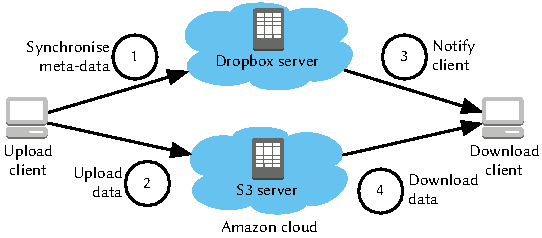
\includegraphics[width=\columnwidth]{application/cloud_file_synchronization/system_model/figures/dropbox_architecture}
  \caption{\dropbox file storage and retrieval process}
  \label{fig:application:cloud_file_synchronisation:system_model:dropbox_architecture}
\end{figure}

The \dropbox infrastructure consists of two main components:
\begin{enumerate*}
\item a storage cloud based on Amazon's Elastic Compute Cloud and Simple Storage Service, and 
\item (2) control servers directly maintained by \dropbox Inc. 
\end{enumerate*}

The control servers store meta information about the current state of the files in the \dropbox folders and trigger synchronization processes on the clients.

A file synchronization can basically be described in five steps.
As soon as the new file is added to the \dropbox folder of the uploading client, a preprocessing step is triggered and the meta information for the file are generated, respectively updated.
This information is then synchronized with the control servers~(1) and the file itself is uploaded to the storage cloud~(2).
After the file has completely been transferred to the storage cloud, all connected clients are notified about the update~(3) and start downloading the new file~(4).

\subsubsection*{Use Case: Photo Uploading}\label{sec:application:cloud_file_synchronisation:use_case}
In this section we consider the synchronization of images from a digital camera to a mobile \gls{UE} via a cloud storage provider.
Real world examples of this scenario are, e.g., taking photos of a live event and transferring them to a picture agency, or shooting private holiday images. 

The user took a finite set of pictures with a wearable device like Google Glass or a smart camera, e.g. a Nikon Coolpix S800c or SAMSUNG CL80.
The camera is then connected via a \gls{PAN} with a mobile \gls{UE}, for example a Laptop with a data card or a smartphone, to store the images on the mobile device.
The \gls{UE} uses broadband wireless Internet access technology and runs software provided by the cloud storage provider in order to synchronise the images with the cloud storage.
Finally, the scenario includes a remote client, which is connected using a wire line connection and downloads the images from the cloud.

For the evaluation presented in this paper, we consider a specific realization of the use case described above.
For the role of the cloud storage provider we consider \dropbox, Bluetooth is used as the technology for establishing the \gls{PAN}, and \gls{LTE} is used as the wireless broadband access technology.

In the considered scenario the interests of two stakeholders are impacted.
The first stakeholder, the end user, has two contradicting requirements on the system.
On the one hand side, the images should be synchronised as fast as possible. 
This requires a fast and permanent Internet connection of the \gls{UE}, which in turn is very power intensive.
On the other side, the power drain of the mobile device should be minimized to enable a long battery life time.
The second stakeholder, the mobile network provider, wants to minimize the signallisation overhead in the network~\cite{NSN2011, Huawei2011} caused by short time connections.
Here, an optimisation problem arises to find a practical solution for all three requirements. 
In order to analyse this problem, we use a simulation model of the file synchronization process, which is described in the following.

\subsubsection*{Cloud Storage Model and Performance Metrics}\label{sec:application:cloud_file_synchronisation:system_model:model_metrics}
The proposed simulation model is schematically depicted in \reffig{fig:application:cloud_file_synchronisation:system_model:model_metrics:model} and based on the findings of~\cite{Drago2012} described in~\refsec{sec:application:background}.

\begin{figure}
\centering
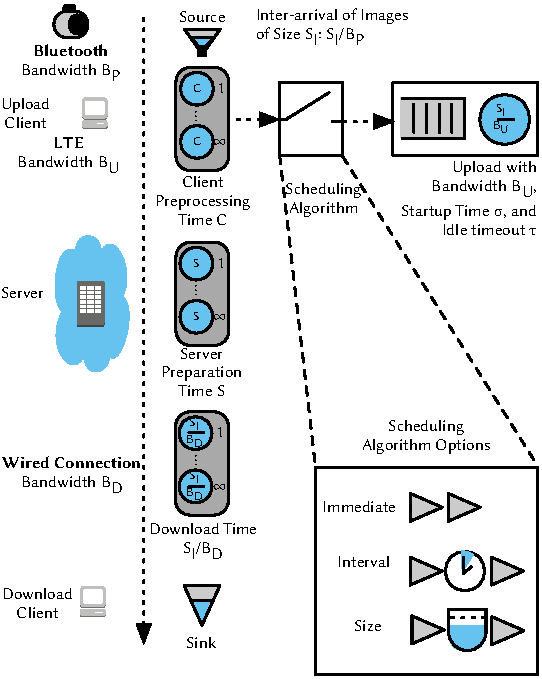
\includegraphics[width=\columnwidth]{application/cloud_file_synchronization/system_model/figures/model}
\caption{Synchronization Process Model}
\label{fig:application:cloud_file_synchronisation:system_model:model_metrics:model}
\end{figure}

We assume that the user has taken pictures of varying file size distributed with \imageFileSize.
These pictures are transfered from the camera to the mobile device using the \gls{PAN} with a constant bandwidth~\panTransferRate.
Due to the limited bandwidth \panTransferRate of the \gls{PAN} device, the inter-arrival times of images at the \dropbox shared folder of the mobile device can be calcluated by \(\interarrivaltime = \frac{\imageFileSize}{\panTransferRate}\).

As soon as the image is fully copied to the \dropbox folder, the generation of the meta data introduces a preprocessing delay, which we refer to as client preparation time~\clientpreparationtime.
To evaluate different strategies optimising the overall waiting time, power drain, and signallisation traffic we include a scheduling component.
This component implements different algorithms, described in \refsec{sec:application:cloud_file_synchronisation:system_model:algorithms}, which decide when the images currently held available in the scheduling component should be sent to the component responsible for transmission.

Next, we consider the \gls{LTE} \gls{UE} used for image upload.
Due to the specification of the \gls{LTE} standard \cite{3GPP_RRC_Spec}, the upload component can, at any point in time, either be connected to the mobile network or disconnected.
If the \gls{UE} is currently disconnected, and a new image for upload arrives, the connection process is triggered and completed after a startup delay \(\startupDelay = \SI{0.26}{\second}\).
Once the \gls{UE} is connected, arriving images are transmitted in order.
The transmission, i.e. service time, of an image depends on the size of the image currently being uploaded as well as the upload bandwidth \uploadbandwidth.
As only one image is transferred at once, waiting images are stored in a queue of infinite size.
If the \gls{UE} is idle for more than \(\idleThreshold = \SI{11.576}{\second}\), the device disconnects from the network.

After the image has been successfully uploaded to the storage servers, a server side preprocessing phase starts, before the file transfer to the downloading client starts.
This server side preprocessing again introduces an additional delay, the server preparation time~\serverpreparationtime, in the synchronization process.
Finally, the image is downloaded by the wire line client.
Again, the duration is calculated based on the size of the image and the available download bandwidth~\downloadbandwidth.

Next, we discuss the metrics used to evaluate the performance of the scheduling algorithms under consideration.
First, we consider the mean synchronization time \sojournTime, i.e., the time between the generation of images and the completion of the download.
This metric accounts for the desire of end users to synchronize images in a short amount of time.
Secondly, we study the relative amount of time the \gls{UE} is disconnected \relativeDisconnectedTime.
As the \gls{UE} consumes more power in the connected state, the user is generally interested in scheduling mechanisms which ensure that the device is only connected if required \cite{Ickin2012}.
This measure also enables a more general evaluation then the actually consumed power, as the concrete power drain differs significantly for each device.
Finally, we evaluate the number of transitions~\connectionCount between the connected and disconnected states.
As discussed in \refsec{chap:network}, frequent state transitions put a strain on the network due to increased signallling.
Thus, scheduling algorithms with a small number of transitions would be favored by network operators.

\subsubsection*{Scheduling Algorithms}\label{sec:application:cloud_file_synchronisation:system_model:algorithms}
We use different scheduling strategies in our model to control the uploading of the files from the mobile client.
These mechanisms in turn affect the synchronization time, the power drain, and the generated signalling traffic.

The most basic strategy of handing the upload is to immediately send new files, as soon as the meta data is generated.
We refer to this as \algoimmediate strategy and will use this as base line for all comparisons in the evaluations.
The other two strategies considered are based on a temporal, respectively a size threshold. 
Using the \algointerval scheduling, the client checks periodically if new files have been marked for synchronization.
If new files are present, they are synchronized to \dropbox.
Files which could not be sent within the current interval will automatically be added to the file batch for the next interval. 
The last scheduling mechanisms uses a threshold based on the overall \algosize of the images not yet synchronized.
If the threshold is crossed, an upload is triggered.

\subsection{YouTube \headershortacr{QoE} Model}\label{sec:application:qoe_user_behaviour:typical_user_scenarios:youtube_qoe}
This section introduces \gls{QoE} models for YouTube video playback.
First, we extend the \gls{QoE} mapping function introduced in~\cite{Hossfeld2013c} in order to support user preferences regarding sensitivity to stalling duration and number of stalling events.
Then, we provide a parametrised mapping function allowing for user preferences regarding initial delay.
Finally, we combine the proposed mapping functions.

\subsubsection*{Stalling \headershortacr{QoE} Model}\label{sec:application:qoe_user_behaviour:typical_user_scenarios:youtube_qoe:stalling}
The \gls{QoE} of \gls{HTTP} streaming depends mainly on the actual number of stalling events \(N\) for a video of duration \(T\) and the average length \(L\) of a single stalling event.
A \gls{QoE} model combining both key influence factors into a single equation \(f(L,N)\) is provided in~\cite{Hossfeld2013c} and found to follow the IQX hypothesis~\cite{Fiedler2010} describing an exponential relationship between the influence factors and \gls{QoE}.
In particular, the model function returns \gls{MOS} on a 5-point absolute category rating scale with 1 indicating the lowest \gls{QoE} and 5 the highest \gls{QoE}. 
\begin{equation}
 f(L,N) = 3.5 e^{-(0.15L + 0.19)N}+1.50
\label{eq:application:qoe_user_behaviour:typical_user_scenarios:youtube_qoe:stalling:original_model}
\end{equation}
Due to well known rating scale effects, the model in \refeq{eq:application:qoe_user_behaviour:typical_user_scenarios:youtube_qoe:stalling:original_model} has a lower bound of \(1.50\), as users avoid the extremities of the scale called \emph{saturation effect}, see e.g.~\cite{Moller2000}.
In contrast, if the video is not stalling, no degradation is observed and users rate the impact of stalling as 'imperceptible', i.e. a value of 5.

It has to be noted that the model function in \refeq{eq:application:qoe_user_behaviour:typical_user_scenarios:youtube_qoe:stalling:original_model} is based on subjective user studies with videos of duration up to \(T=\SI{30}{\second}\).
For other video durations, the normalized number \(N^*=\frac{N}{T}\) of stalling events has to be considered which requires to adapt the parameters \(\alpha=0.15\) and \(\beta=0.19\) in \refeq{eq:application:qoe_user_behaviour:typical_user_scenarios:youtube_qoe:stalling:original_model}, respectively. 

As the goal of our investigation is the analysis of the impact of different user profiles, we parametrize the function in \refeq{eq:application:qoe_user_behaviour:typical_user_scenarios:youtube_qoe:stalling:original_model} with parameters \(\alpha\) and \(\beta\) and conduct a parameter study on their impact. 
For the sake of simplicity, we normalize the QoE value to be in the range \(\left[0;1\right]\)  and use the normalized number of stalling events $N^*$. 
As a result, we arrive at \refeq{eq:application:qoe_user_behaviour:typical_user_scenarios:youtube_qoe:stalling:parameterized_model} as parametrized \gls{QoE} model \(Q_1\) to quantify the impact of stalling on QoE for different user profiles expressed by \(\alpha\) and \(\beta\). 
Thereby, the parameter \(\alpha\) adjusts the sensitivity of the user to the stalling duration \(L\cdot N^*\), while \(\beta\) quantifies the sensitivity of the user to the actual number of stalling events, i.e. the video interruptions.
Therefore, we will also use the term \emph{duration parameter} and \emph{interruption parameter} for \(\alpha\) and \(\beta\), respectively.

\begin{equation}
   Q_1(L,N^*) = e^{-\left( \alpha L + \beta\right) N^*} 
\label{eq:application:qoe_user_behaviour:typical_user_scenarios:youtube_qoe:stalling:parameterized_model}
\end{equation}

The model function \(Q_1\) in \refeq{eq:application:qoe_user_behaviour:typical_user_scenarios:youtube_qoe:stalling:parameterized_model} has the same form as \refeq{eq:application:qoe_user_behaviour:typical_user_scenarios:youtube_qoe:stalling:original_model} and follows the IQX hypothesis, but allows to investigate different user profiles.
For example, some users may suffer stronger from interruptions which is then adjusted by a higher value of \(\beta\).
Thus, a user profile can be expressed in terms of different values of the duration parameter \(\alpha\) and the interruption parameter \(\beta\)

\subsubsection*{Initial Delay \headershortacr{QoE} Model}\label{sec:application:qoe_user_behaviour:typical_user_scenarios:initial_delay}
Another impairment on \gls{HTTP} streaming \gls{QoE} are initial delays before the video playout can start for the first time.
The impact of initial delays \(T_0\) is modeled by the function given in \refeq{eq:application:qoe_user_behaviour:typical_user_scenarios:initial_delay:original_model}, model parameters are obtained from subjective tests \cite{Hossfeld2012c}. 
\begin{equation}
g(T_0)=-0.963 \mathrm{log10}(T_0 + 5.381) + 5
\label{eq:application:qoe_user_behaviour:typical_user_scenarios:initial_delay:original_model}
\end{equation}

The results in~\cite{Hossfeld2012c} show that the impact of the initial delay is independent of the video duration which was either \SI{30}{\second} or \SI{60}{\second} in the user tests.
Further, it was observed that users have a clear preference of initial delays instead
of stalling and that service interruptions have to be avoided in any case, even at costs of increased initial delays for filling up the video buffers. 

For the sake of simplicity, we normalize the function in \refeq{eq:application:qoe_user_behaviour:typical_user_scenarios:initial_delay:original_model} to obtain the \gls{QoE} model \(Q_2\) for initial delays \(T_0\), so that \(Q_2\) returns values in \(\left[0;1\right]\) and that \(Q_2(0)=1\) holds, by adding the term \(\gamma \mathrm{log10}\left(c\right)\).

The user profile is parametrized with the parameter \(\gamma\) determining the impact of initial delays on the user \gls{QoE}.
The constant \(c=5.381\) is taken from \refeq{eq:application:qoe_user_behaviour:typical_user_scenarios:initial_delay:original_model} defining the shape of the curve. 
Since the logarithm is not bounded, only positive values are considered to ensure \(Q_2(T_0) \in [0;1]\).
\begin{equation*}
Q_2(T_0)= -\gamma \mathrm{log10}\left(T_0 + c\right) + \gamma \mathrm{log10}\left(c\right)+ 1 
\end{equation*}

\subsubsection*{Combined \headershortacr{QoE} Model}\label{sec:application:qoe_user_behaviour:typical_user_scenarios:youtube_qoe:combined}
For dimensioning the video buffers, we are interested in a \gls{QoE} model which considers both, the impairments due to stalling and due to initial delays of the video playout.
However, to the best of our knowledge no combined model exists so far which has been validated by proper subjective user studies.
Therefore, we suggest the following model \(Q\).
Since the impact of stalling events clearly dominates the user perception \cite{Hossfeld2012a,Hossfeld2012c}, we consider the following rationale for the combined QoE model.
A user facing an initial delay \(T_0\) experiences a \gls{QoE} value of \(Q_2(T_0)\).
If additional stalling events occur, this will lower the QoE further.
Thus, \(Q_2(T_0)\) is the upper bound of \gls{QoE}.
For \(N^*\) stalling events with an average length \(L\), the \gls{QoE} will be further decreased by \(Q_1(L,N^*)\).

An additive \gls{QoE} model for non-adaptive HTTP streaming which is referred to as buffer-related perceptual indicator is recommended in \cite{ITUT2012}. This model follows the same rationale above, start from the maximum QoE value which is \(1=Q(0,0,0)\), subtract the degradation from stalling \(1-Q_1(L,N^*)\) and \(1-Q_2(T_0)\) stemming from initial delay.

Then, we arrive at the following additive QoE model \(Q\) used in the following analysis.  
\begin{eqnarray}
  Q(T_0,L,N^*) &=& 1-(1-Q_1(L,N^*)) - (1-Q_2(T_0)) \notag\\
   &=& Q_1(L,N^*) + Q_2(T_0) - 1
\label{eq:application:qoe_user_behaviour:typical_user_scenarios:youtube_qoe:combined:qsum}
\end{eqnarray}

\subsection{\headershortacr{QoE} Study for Typical User Scenarios}\label{sec:application:qoe_user_behaviour:typical_user_scenarios}
Based on the playback model introduced in \refsec{sec:application:qoe_user_behaviour:system_model} and the parametrised \gls{QoE} user model proposed in \refsec{sec:application:qoe_user_behaviour:typical_user_scenarios:youtube_qoe}, this section studies three typical user scenarios.
We discuss optimal choices for buffer size depending on user preferences and highlight the impact of buffer choices neglecting the user preference.

\subsubsection*{Watch later Scenario}\label{sec:application:qoe_user_behaviour:typical_user_scenarios:watch_later}
In the \watchLater scenario, a user requests a video, but the user does not expect that the video playout starts immediately. 
This may be the case for example when the user wants to watch an HD at a later time and expects low network bandwidth. 
During that initial delay, the user may opt do something else, e.g. opening another web page in a parallel tab in the browser.
Thus, \gls{QoE} is not affected by initial delays and we only need to consider \(Q_1\) in \refeq{eq:application:qoe_user_behaviour:typical_user_scenarios:youtube_qoe:stalling:parameterized_model}.

In the steady state, we have \(L=\frac{d}{\lambda}\) and \(N^*=\frac{\mu-\lambda}{d}\) and we obtain the following QoE relation in \refeq{eq:application:qoe_user_behaviour:typical_user_scenarios:stalling_steady_state}. 

\begin{equation}
   Q_1(L,N^*) = e^{\left(\mu-\lambda\right)(\frac{\alpha}{\lambda} +\frac{\beta}{d^*})}
	 = e^{-\alpha \frac{1-a}{a} - \beta \frac{1-a}{d^*}}
\label{eq:application:qoe_user_behaviour:typical_user_scenarios:stalling_steady_state}
\end{equation}

Since the \gls{QoE} function in \refeq{eq:application:qoe_user_behaviour:typical_user_scenarios:stalling_steady_state} is strictly monotonically increasing in the normalized buffer size \(d^*\), the optimum is achieved for 
\[Q_+=\lim\limits_{d^* \to \infty} Q_1(L,N^*)=e^{-\alpha \frac{1-a}{a}}.\]
Thus, the QoE value only depends on the parameter \(\alpha\) in the limit.
To see for which buffer size we are close to the optimum, we consider the relative difference \(\frac{Q_+-Q_1(L,N^*)}{Q_+}\) when it is less than \(\Omega=\SI{5}{\percent}\).
This is true for any \(d^*> -\beta \frac{1-a}{\log\left(1-\Omega\right)}\). 

For \(\beta \in \{0.05,0.2\}\), a small buffer size of \(d^*>\SI{4}{\second}\) is already sufficient to be close to the optimum \(Q_+\) for any offered network condition \(a\).
For users extremely sensitive to stalling, e.g. for \(\beta=0.8\), buffer sizes up to \SI{15}{\second} are required.
However, a buffer of \SI{4}{\second} is sufficient for a relative difference to the optimum of \SI{20}{\percent}. 
In general, the larger the buffer size the better the obtained \gls{QoE} is in this scenario. In practice, a buffer size of \SI{4}{\second} is a good choice.

\subsubsection*{Default Video Streaming Scenario}\label{sec:application:qoe_user_behaviour:typical_user_scenarios:default}

In the case of normal streaming, the user wants to watch a video immediately for a long period of time.
In contrast to the \watchLater scenario, the initial delay impacts the \gls{QoE} in the \watchNow scenario according to \refeq{eq:application:qoe_user_behaviour:typical_user_scenarios:youtube_qoe:combined:qsum}.

\begin{figure}
  \centering
  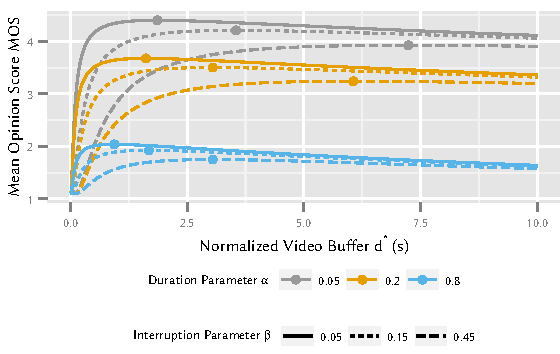
\includegraphics{application/qoe_user_behaviour/user_scenarios/figures/default_scenario}
  \caption{Dimensioning of buffer size in the \emph{Streaming Scenario} for available network bandwidth of \(a = 0.5\). Maxima marked as dots mainly depend on \(\beta\).}
  \label{fig:application:qoe_user_behaviour:typical_user_scenarios:default:default_scenario}
\end{figure}

\reffig{fig:application:qoe_user_behaviour:typical_user_scenarios:default:default_scenario} shows \gls{QoE} depending on the buffer size \(d^*\) for the \watchNow scenario and different user profiles in a network situation \(a=0.5\) leading to a stalling ratio \(R=0.5\).

Now, \gls{QoE} optima exist for finite buffer size, if the impact of the initial delay is taken into consideration. 
We notice that \(\alpha\) does increase the \gls{QoE} but has no significant impact on the optimal buffer size.
In contrast, for different \(\beta\) we observe different optima for the buffer size.
Therefore, we can neglect the interruption parameter \(\alpha\) when optimising the buffer size with regard to the \gls{QoE}.
A buffer size less than \SI{0.5}{\second} results in a severe loss of \gls{QoE} for all users.
A buffer size of \SIrange{2}{4}{\second} offers a good \gls{QoE} for the average user and any sensitive user.
Increasing the buffer size further decreases the \gls{QoE}.

\subsubsection*{Video Browsing Scenario}\label{sec:application:qoe_user_behaviour:typical_user_scenarios:browsing}

In the case of the \videoBrowsing scenario, the user watches a video for a short period of time. This includes cases such as, viewing a short video completely, viewing a short part of a long video or skipping ahead in a video frequently, thus watching multiple short parts of a video.
In this scenario, a steady state can not be assumed due to the short watching duration.
Since we know from the previous section that \(\alpha\) and \(\beta\) have only a marginal impact on the optimal \gls{QoE}, we consider only the default parameters \(\alpha=0.15\) and \(\beta=0.2\) in the following.
However, for video browsing, the impact of the initial delay may be more important for the user. Therefore, we consider two different types of delay sensitive users with \(\gamma=0.2\) as well as a more delay sensitive user with \(\gamma=0.8\).

\begin{figure}
  \centering
  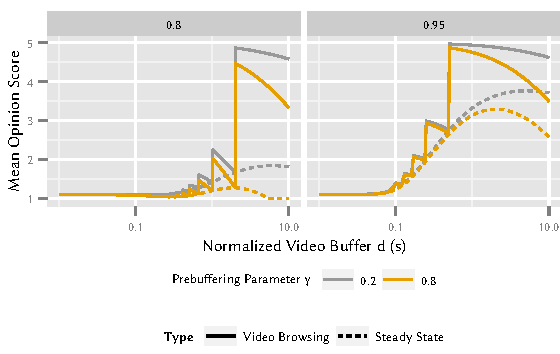
\includegraphics{application/qoe_user_behaviour/user_scenarios/figures/video_browsing}
  \caption{Dimensioning of buffers for \emph{Video Browsing} users with varying \gls{QoE} sensitivity to initial delays. Users abort the video after \SI{10}{\second}.}
  \label{fig:application:qoe_user_behaviour:typical_user_scenarios:browsing:video_browsing}
\end{figure}

In \reffig{fig:application:qoe_user_behaviour:typical_user_scenarios:browsing:video_browsing}, the impact of the buffer size on the \gls{QoE} is depicted for the case that the video is aborted after the first \SI{10}{\second} using a logarithmic x-axes. 
We consider two different network scenarios with an offered load of \(a = 0.8\) and \(a = 0.9\).
Multiple local QoE maxima exist independently of \(\gamma\), which appear when the number of stalling events change. 
For different values of \(\beta\) these maxima occur at the same buffer size.
Therefore, we can ignore \(\beta\) in this scenario. 
The local minima exist at the buffer size for which the last stalling event has the smallest possible length. 
The results for the steady state are also included and we observe that the steady state provides a lower bound for the finite buffer results.

Thus, the steady state can be used to perform worst case buffer dimensioning.
For very low offered loads \(a\), e.g. \(a = 0.1\) which is not shown due to scale, the \gls{QoE} is very low for both, the steady state and the finite case. 
Thus, video streaming and especially \videoBrowsing is not desirable in this case. 
However, for larger buffer sizes, the difference between the local maxima and the steady state increases. 
Nevertheless, in those cases, the initial delay exceeds tens of seconds.
So this scenario can not be described as realistic \videoBrowsing.

In general, if the exact viewing length of a video was known, e.g. short videos will be watched completely, the buffer size could be set so that the \gls{QoE} lies at a local maximum which is independent of \(\gamma\).
However, this method can result in a severe loss of \gls{QoE}, depending on \(\gamma\) if the user aborts earlier, as the actual \gls{QoE} loss significantly depends on \(\gamma\). 
In practice, a buffer size of \SIlist{1;2}{\second} is recommended for video browsing. 
If the buffer size is set too large, \(\gamma\) determines again the actual \gls{QoE} loss.
For larger buffer sizes, the sensitivity \(\gamma\) to initial delays strongly influence the \gls{QoE}.